
%% version 0.0 Alpha

%% see airavata.me/about
%% for current contact information.

\documentclass[conference,a4paper,american]{IEEEtran}
\usepackage{blindtext}
\usepackage{graphicx}
\usepackage{float}
\usepackage{hyperref}
\usepackage{nameref}
\usepackage{multirow}
\usepackage{graphicx}
\usepackage{array}
\usepackage{tabularx}
\usepackage{tabulary}
\usepackage{ltxtable} %for long table
\usepackage{etoolbox}
\usepackage{slantsc}
\usepackage{url}
%\usepackage[style=authoryear,backend=biber]{biblatex}
\usepackage{booktabs}% http://ctan.org/pkg/booktabs
\let\labelindent\relax


% \let\author\relax % please?


\usepackage{enumitem}

%\usepackage{caption}
% \usepackage{lon} %for long table

\usepackage{xcolor} %start packages for colored code listing
\usepackage{upquote} %start packages for colored code listing

% \usepackage{apacite} % for APA citing style
\usepackage{wrapfig} %untuk wrapfigure?
%reconfiguring inline list
\newlist{inlinelist}{enumerate*}{1}
\setlist*[inlinelist,1]{
	label={\alph*)},font={\color{red!50!black}\bfseries}
}

\hyphenation{op-tical net-works semi-conduc-tor}

\begin{document}
	
\title{Optimasi Kasiski Examination pada Studi Kasus SPOJ The Bytelandian Cryptographer (Act IV)}{Optimization Kasiski Examination on Study Case SPOJ The Bytelandian Cryptographer (Act IV)}{KI141502} 

% \author{Nama Lengkap}{NRP}
\author{Freddy Hermawan Yuwono}{5113100040}

% \supervisorOne{Nama Pembimbing Satu}{NIP}
% \supervisorTwo{Nama Pembimbing Dua}{NIP}
\supervisorOne{Rully Soelaiman, S.Kom, M.Kom}{197002131994021001}
\supervisorTwo{Wijayanti Nurul Khotimah, S.Kom., M.Sc}{198603122012122004}

% \degree{Nama Gelar}{Bidang Studi}{Program Studi}{Jurusan}{Jurusan (English)}{Fakultas}{Fakultas Singkatan}{Fakultas (English)}
\degree{Sarjana Komputer}{Algoritma Pemrograman}{S1}{Teknik Informatika}{Informatics}{Teknologi Informasi}{FTIf}{Information Technology}

% \time{bulan}{tahun}
\time{Desember}{2017}

	
	
\begin{abstract}
	
	Pada Era Digitalisasi ini, tingkat kebutuhan masyarakat akan informasi semakin meningkat. Hal ini menyebabkan pertukaran informasi menjadi sangat mudah. Hal ini membuat informasi yang bersifat sensitif dapat terjadi kebocoran informasi kepada pihak - pihak yang tidak berkepentingan. Kebocoran informasi terbagi menjadi 2 apabila dilihat dari keutuhan informasi yang didapat, yaitu sebagian dan seutuhnya. Kebocoran informasi yang bersifat sebagian, membuat pihak-pihak yang tidak berkepentingan tetapi yang meminginkan informasi tersebut, berusaha untuk mendapatkan informasi yang utuh dari potongan-potongan informasi yang telah didapatkan.
	\newline
	 Permasalahan dalam buku tugas akhir ini adalah permasalahan untuk mendapatkan \textit{plaintext} sebanyak-banyaknya dari \textit{ciphertext} dan batas atas panjang kunci pada metode enskripsi yang menggunakan teknik \textit{Vigenere Cipher}. Dalam permasalahan ini diberikan \textit{plaintext} dan \textit{ciphertext}, akan tetapi terdapat informasi yang hilang pada keduanya. Diberikan batas atas panjang kunci, dimana batas atas ini belum tentu panjang kunci yang sesungguhnya. Untuk dapat merekonstruksi \textit{plaintext} dari kepingan informasi yang didapatkan diperlukan untuk mencari panjang kunci yang di dapatkan dengan cara memodifikasi \textit{Kasiski Examination} dan \textit{Intersection}. Beberapa hal yang perlu diperhatikan seperti mempercepat dari \textit{Kasiski Examination} dan juga \textit{Intersection} terhadap hasil yang diperoleh dari pencarian panjang kunci.
	\newline 
	\indent Hasil dari tugas akhir ini telah berhasil untuk menyelesaikan permasalahan yang telah diangkat dengan benar. Waktu yang diperlukan untuk dapat menyelesaikan masukan sebesar 2MB dalam 4,42 detik dengan alokasi memori sebesari 26,5MB.\\
\end{abstract}
% IEEEtran.cls defaults to using nonbold math in the Abstract.

\begin{IEEEkeywords}
\textit{Plaintext}, \textit{Ciphertext}, \textit{Kasiski Examination},  Optimisasi.
\end{IEEEkeywords}

\IEEEpeerreviewmaketitle

	\section{Pendahuluan}
Ketergantungan seseorang terhadap informasi tidak terlepas dari kebutuhan manusia akan informasi yang berada disekitarnya. Informasi yang diterima seseorang pada masa sekarang dapat melalui media fisik dan media digital. Media fisik seperti koran dan majalah, sedangkan media digital seperti facebook dan twitter. Media-media tersebut sanggup untuk menyebarkan informasi sangat cepat, sehingga orang-orang dengan cepat mengetahui informasi yang berada disekitarnya.
\\
\indent Informasi digital yang beredar di dunia maya pun tidak lepas dari penyalahgunaan informasi. Dibutuhkan suatu teknik penyandian terhadap data yang dimiliki agar data yang bersifat rahasia itu tidak diketahui dengan orang – orang yang tidak berkepentingan.Akan tetapi hal ini menarik perhatian dari pihak-pihak yang mengingkan informasi tersebut tetapi informasi yang diperoleh hanyalah terbatas dengan kepingan-kepingan saja. Seperti contohnya adalah studi kasus SPOJ \textit{The Bytelandian Cryptographer(Act IV)}. Pada studi kasus ini diketahui bahwa metode enskripsi yang digunakan adalah \textit{Vigenere Cipher}. Diberikan sejumlah kasus ujicoba, dimana pada setiap kasus ujicoba diberikan sejumlah potongan-potongan informasi dari \textit{plaintext} dan \textit{ciphertext}, batas atas dari panjang kunci yang digunakan(Panjang Kunci yang diberikan bukan panjang kunci yang sesungguhnya). Diharapkan dari studi kasus tersebut adalah merekonstruksi ulang \textit{plaintext} dari apa yang telah tersedia. Batasan masalahnya dimana jumlah inputan tidak akan melebihi dari 2 MB, batas atas panjang kuncinya bernilai $1<=M<=100,000$, dan jumlah kasus ujicoba $1<=T<=200$. Solusi dari studi kasus yang akan dibahas akan diimplementasikan dalam bentuk kode. 
\\
\indent Hasil dari Tugas Akhir ini diharapkan dapat merekonstruksi ulang pesan dari kepingan-kepingan informasi yang telah didapatakan sebelumnya. Sehingga diharapkan memberikan kontribusi pada pengembangan ilmu pengetahuan dan komunikasi. 
% \subsection{Subsection Heading Here}
% \blindtext

	
\section{Tinjuan Pustaka}

\subsection{\textit{Kasiski Examination}}
\textit{Kasiski Examination} adalah suatu teknik yang digunakan untuk mencari panjang kunci dari suatu \textit{ciphertext} dari suatu \textit{Polyalphabetic Cipher} dan turunannya, dengan memanfaatkan kelemahan dari \textit{Polyalphebetical Cipher}, tanpa harus mengetahui \textit{plaintext} dan himpunan kunci yang digunakan. Kelemahaannya yaitu dimana apabila suatu \textit{substring} \textit{plaintext} yang sama dienskripsi dengan \textit{substring} dari kunci yang digunakan akan menghasilkan pola yang sama\cite{noauthor_kasiski_nodate}. Metode pencarian panjang kunci yang dilakukan adalaha sebagai berikut.
\begin{enumerate}
\item Mencari semua \textit{substring} yang berulang pada suatu kalimat.
\item Mencari panjang dimana \textit{subtring} tersebut berulang kembali.
\item Mencari semua faktor dari nilai yang diperoleh dari tahap 2.
\item Mencari faktor persekutuan terbesar dari hasil yang diperoleh pada tahap 3.
\end{enumerate}


\subsection{\textit{Intersection}}
\textit{Intersection} adalah himpunan $A$ dan himpunan $B$, dimana ada bagian dari $A$ juga merupakan bagian dari $B$. \cite{devlin_joy_1993}.


	% si deskripsi sistem masuk subsistem sebelumnya
	% jadi subsection
	\section{Metode Penyelesaian}
\label{chap:selesai}
Dalam bagian pendahuluan telah dijelaskan bahwa enskripsi yang digunakan adalah \textit{Vigenere Cipher}. Dimana enskripsi yang dilakuakn mengikuti aturan 
\begin{equation}
	y_i=x_i+k_{1+(i-1)mod M} mod 26 
\end{equation}
Pada studi kasus inputan yang bernilai A sampai dengan Z, dapat direpresentasikan menjadi $0$ sampai dengan $25$. 
Tahapan-tahapan untuk menyelesaikan studi kasus ini sebagai berikut:
\begin{enumerate}
\item Menyimpan posisi indeks karakter, dimana pada indeks tersebut baik \textit{ciphertext} maupun \textit{plaintext} tidak bernilai "*", besertra menyimpan hasil perhitungan selisih antara \textit{ciphertext} dan \textit{plaintext}  \cite{john_jones_spoj_2009}.
	\item Menyimpan posisi indeks, apabila \textit{ciphertext} diketahui dan \textit{plaintext} tidak diketahui. Untuk mengurangi \textit{running time} dari program \cite{john_jones_spoj_2009}.
	\item Pada tahapan ini adalah modifikasi dari \textit{Kasiski Examnination}, apabila menggunakan \textit{Kasiski Examination} pada umumnya yang hanya mencari posisi berulang dari suatu sub kalimat dalam suatu kalimat tidak bisa digunakan untuk menyelesaikan permasalahan ini. Oleh karena itu diubah menjadi mengiterasi $M$ dari 1 sampai dengan $M$, yang akan digunakan untuk membagi selisih yang diketahui antara \textit{plaintext} dan \textit{ciphertext} sebesar posisi iterasi yang telah berjalan. Melihat apakah dalam blok-blok yang telah terbentuk ini terdapat \textit{collision} dan indeks yang saling bertabrakan memiliki nilai yang sama atau tidak. Apabila sama maka tidak terjadi tabrakan sebalik jika terjadi tabrakan maka harus mencari panjang kunci yang baru. Mengiterasi panjang kunci dari $\frac{M}{2}+1<=N<=M$, alasannya dimulai dari $\frac{M}{2}+1$ tidak dari $1$ karena apabila suatu panjang kunci bernilai benar maka kelipatan dari panjang kunci itu pun juga pasti benar dan untuk mempersingkat waktu \textit{running time} yang seharusnya terjadi. Pada bagian ini dilakukan untuk mencari panjang kunci yang benar dengan cara mengiterasi hasil yang diperoleh pada tahap satu dimodulo dengan posisi iterasi yang dilakukan. Apabila tidak terjadi konflik maka panjang kunci tersebut benar jika sebaliknya yang terjadi maka panjang kunci tersebut tidak salah. Pada bagian ini memungkinkan bahwa bisa jadi lebih dari satu panjang kunci yang bernilai benar.  
	\item Melakukan \textit{intersection} terhadap himpunan dari kunci yang telah di hasilkan pada tahapan sebelumnya  \cite{john_jones_spoj_2009}. \textit{Intersection} yang dilakukan berada didalam perulangan panjang kunci pada waktu \textit{generate} setiap karakter yang terdapat dalam penyimpanan tahap dua pada panjang kunci tersebut dengan ketentuan sebagai berikut:
	\begin{enumerate}
	\item Panjang kunci harus benar.
	\item Apabila terdapat indeks yang tidak dapat dipastikan isinya maka posisinya harus di buang dari penyimpanan dan hasilnya pasti "*".
	\item Apabila plaintext bernilai "*" dan himpunan kunci yang telah terbentuk tidak kosong pada indeks tersebut, maka \textit{plaintext} akan bernilai sesuai dengan kunci yang terbentuk pada indeks tersebut.
	\end{enumerate} 
\end{enumerate}	

	 
%	
\section{Deskripsi Aplikasi}


\subsection{Subsection Heading Here}
\blindtext
 <-
	\section{Ujicoba dan Analisis}

\subsection{Uji coba Kebenaran}
Uji coba kebenaran dilakukan dengan cara mengumpulkan berkas kode implementasi kedalam daring penilaian online SPOJ. Studi kasus yang diselesaikan adalah \textit{The Bytelandian Cryptographer(Act IV)} dengan code CRYPTO4. Hasil uji kebenaran dan waktu eksekusi program pada situs SPOJ ditunjukkan pada gambar \ref{fig:best}.
\begin{figure}[H]
\centering
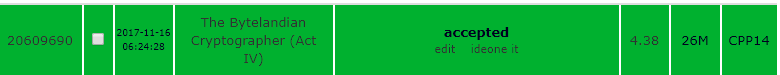
\includegraphics[scale=0.3]{images/best.png}
\caption{Hasil uji kebenaran dengan melakukan submission ke situs penilaian daring SPOJ}
\label{fig:best}
\end{figure}

Uji coba kinerja dari implementasi program yang dihasilkan dengan cara mengumpulkan berkas kode implementasi kedalam daring penilaian online SPOJ sebanyak 30 kali dengan mencatat waktu dan memori yang dibutuhkan, dapat dilihat pada gambar \ref{fig:asf} dan table \ref{tab:statistik}.
\begin{figure}[H]
\centering
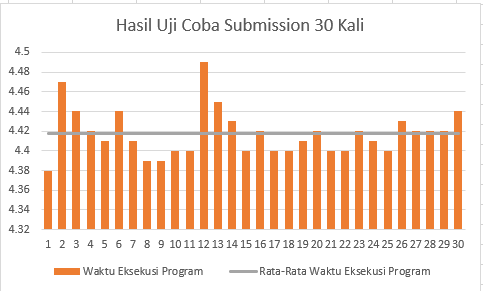
\includegraphics[scale=0.4]{images/uji31.png}
\caption{Hasil Uji Coba Submission ke situs penilaian daring SPOJ sebanyak 30 kali}
\label{fig:asf}
\end{figure}
\begin{table}[H]
	\centering
	\caption{Kecepatan Maksimal, Minimal, dan Rata-Rata dari Hasil Uji Coba Pengumpulan 30 Kali pada Situs Pengujian Daring Spoj}	
	\begin{tabular}{|l|l|} \hline
		Waktu Maksimal & $ 4,49 $ detik\\ \hline
		Waktu Minimal & $ 4,38 $ detik\\ \hline
		Waktu Rata-Rata & $ 4.418 $ detik\\ \hline
		Memori Maksimal & $ 27 $ MB\\ \hline
		Memori Minimal & $ 26 $ MB\\ \hline
		Memori Rata-Rata & $ 26.5 $ MB\\ \hline
	\end{tabular}
	
	\label{tab:statistik}
\end{table}


\subsection{Analisa Kompleksitas}
Berdasarkan algoritma yang telah dibentuk pada bagian metode penyelesaian maka, didapatkan algoritma dengan kompleksitas waktu $\mathcal{O}(T*\frac{M}{2}*(N+S))$ 
	Dimana $n$ adalah panjang karakter \textit{plaintext} atau \textit{ciphertext} , $\frac{M}{2}$ adalah batas atas kunci dibagi dengan 2, $N$ adalah jumlah posisi karakter yang terdapat pada tahap 2 pada subbab \ref{chap:selesai}, dan $S$ adalah jumlah posisi karakter yang terdapat pada tahap 1 pada subbab \ref{chap:selesai}. Pada kondisi \textit{worst case} $T*(N+S)=1.000.000$, sedangakan $\frac{M}{2}$ adalah $50.000$. Hasilnya $50$ miliar perulangan, dengan asumsi $1$ detik adalah $1$ miliar perulangan, maka waktu yang dibutuhkan adalah $50$ detik. Oleh karena itu hal ini tidak mungkin bisa dilakukan begitu saja. Diperlukan pruning pada sumber kode yang ada untuk memangkas waktu eksekusi program. \textit{Prunning} yang dapat dilakukan ketiga menggunakan \textit{Kasiski Examination} dan \textit{Intersection}. Apabila semuanya ini telah dilakukan pasti mendapatkan seperti gambar \ref{fig:best} pada daring online SPOJ.

	%
\section{Introduction}
\blindtext

\subsection{Subsection Heading Here}
\blindtext

	
\section{Kesimpulan}
Dari hasil uji coba yang telah dilakukan terhadap perancangan dan implementasi algoritma untuk menyelesaikan studi kasus SPOJ 20 \textit{The Bytelandian Cryptographer (Act IV)} dapat diambil kesimpulan sebagai berikut:
\begin{enumerate}
 \item Implementasi algoritma dengan menggunakan teknik \textit{Kasiski Examnination} dengan adanya optimasi dapat menyelesaikan permasalahan SPOJ \textit{The Bytelandian Cryptographer (Act IV)} dengan benar.
 \item Kompleksitas waktu $\mathcal{O}(T*\frac{M}{2}*(N+S))$ masih dapat menyelesaikan permasalahan SPOJ \textit{The Bytelandian Cryptographer (Act IV)}
 \item Waktu yang dibutuhkan oleh program untuk menyelesaikan SPOJ \textit{The Bytelandian Cryptographer (Act IV)} minimum $4,38$ detik, maksimum $4,49$ detik dan rata-rata $4.418$ detik. Memori yang dibutuhkan berkisar antara 26-27 MB. %Dibandingkan dengan menggunakan algoritma \textit{Naive} yang memakan waktu jauh lama. Perbandingannya dapat dilihat pada gambar \ref{fig:banding}.
 \end{enumerate}
Saran-saran yang dapat diambil dari metode yang telah di bahas sebagai berikut:
  \begin{enumerate}
    \item Dengan teknik \textit{Kasiski Examination} masih cenderung lambat,karena masih menggunakan teknik \textit{brute force} sehingga hasil yang diperoleh kurang optimal, perlu adanya optimisasi lanjutan yang dapat mencari suatu panjang kunci.%sebenarnya telah dilakukan ujicoba dengan menggunakan bilangan komposit dan bilangan prima yang telah terbentuk dalam persamaan ini, akan tetapi masih menemukan jalan buntu.
    \item Perlu adanya Optimisasi dalam hal pencarian suatu indeks yang perlu dirubah atau tidak. Dengan teknik yang dipakai oleh penulis tidak dapat memenuhi ekspetasi jika berharap dengan hasil yang sangat cepat.
    \end{enumerate}

 
	%	
\appendices
\section{Proof of the First Zonklar Equation}
Some text for the appendix.

	 % use section* for acknowledgement
\section*{Ucapan Terima Kasih}
Puji syukur penulis panjatkan kepada Tuhan Yang Maha Esa atas pimpinan, penyertaan, dan karunia-Nya sehingga penulis dapat menyelesaikan penelitian ini. Penulis juga mengucapkan terima kasih kepada orang tua dan keluarga penulis, juga kepada Bapak Rully Soelaiman dan Ibu Nurul Wijayanti K. selaku dosen pembimbing penulis dan kepada semua pihak yang telah memberikan dukungan baik secara langsung maupun tidak langsung selama penulis mengerjakan penelitian ini.


\ifCLASSOPTIONcaptionsoff
  \newpage
\fi

	\bibliography{Zotero}
	\bibliographystyle{ieeetran}
	%
\begin{IEEEbiography}[{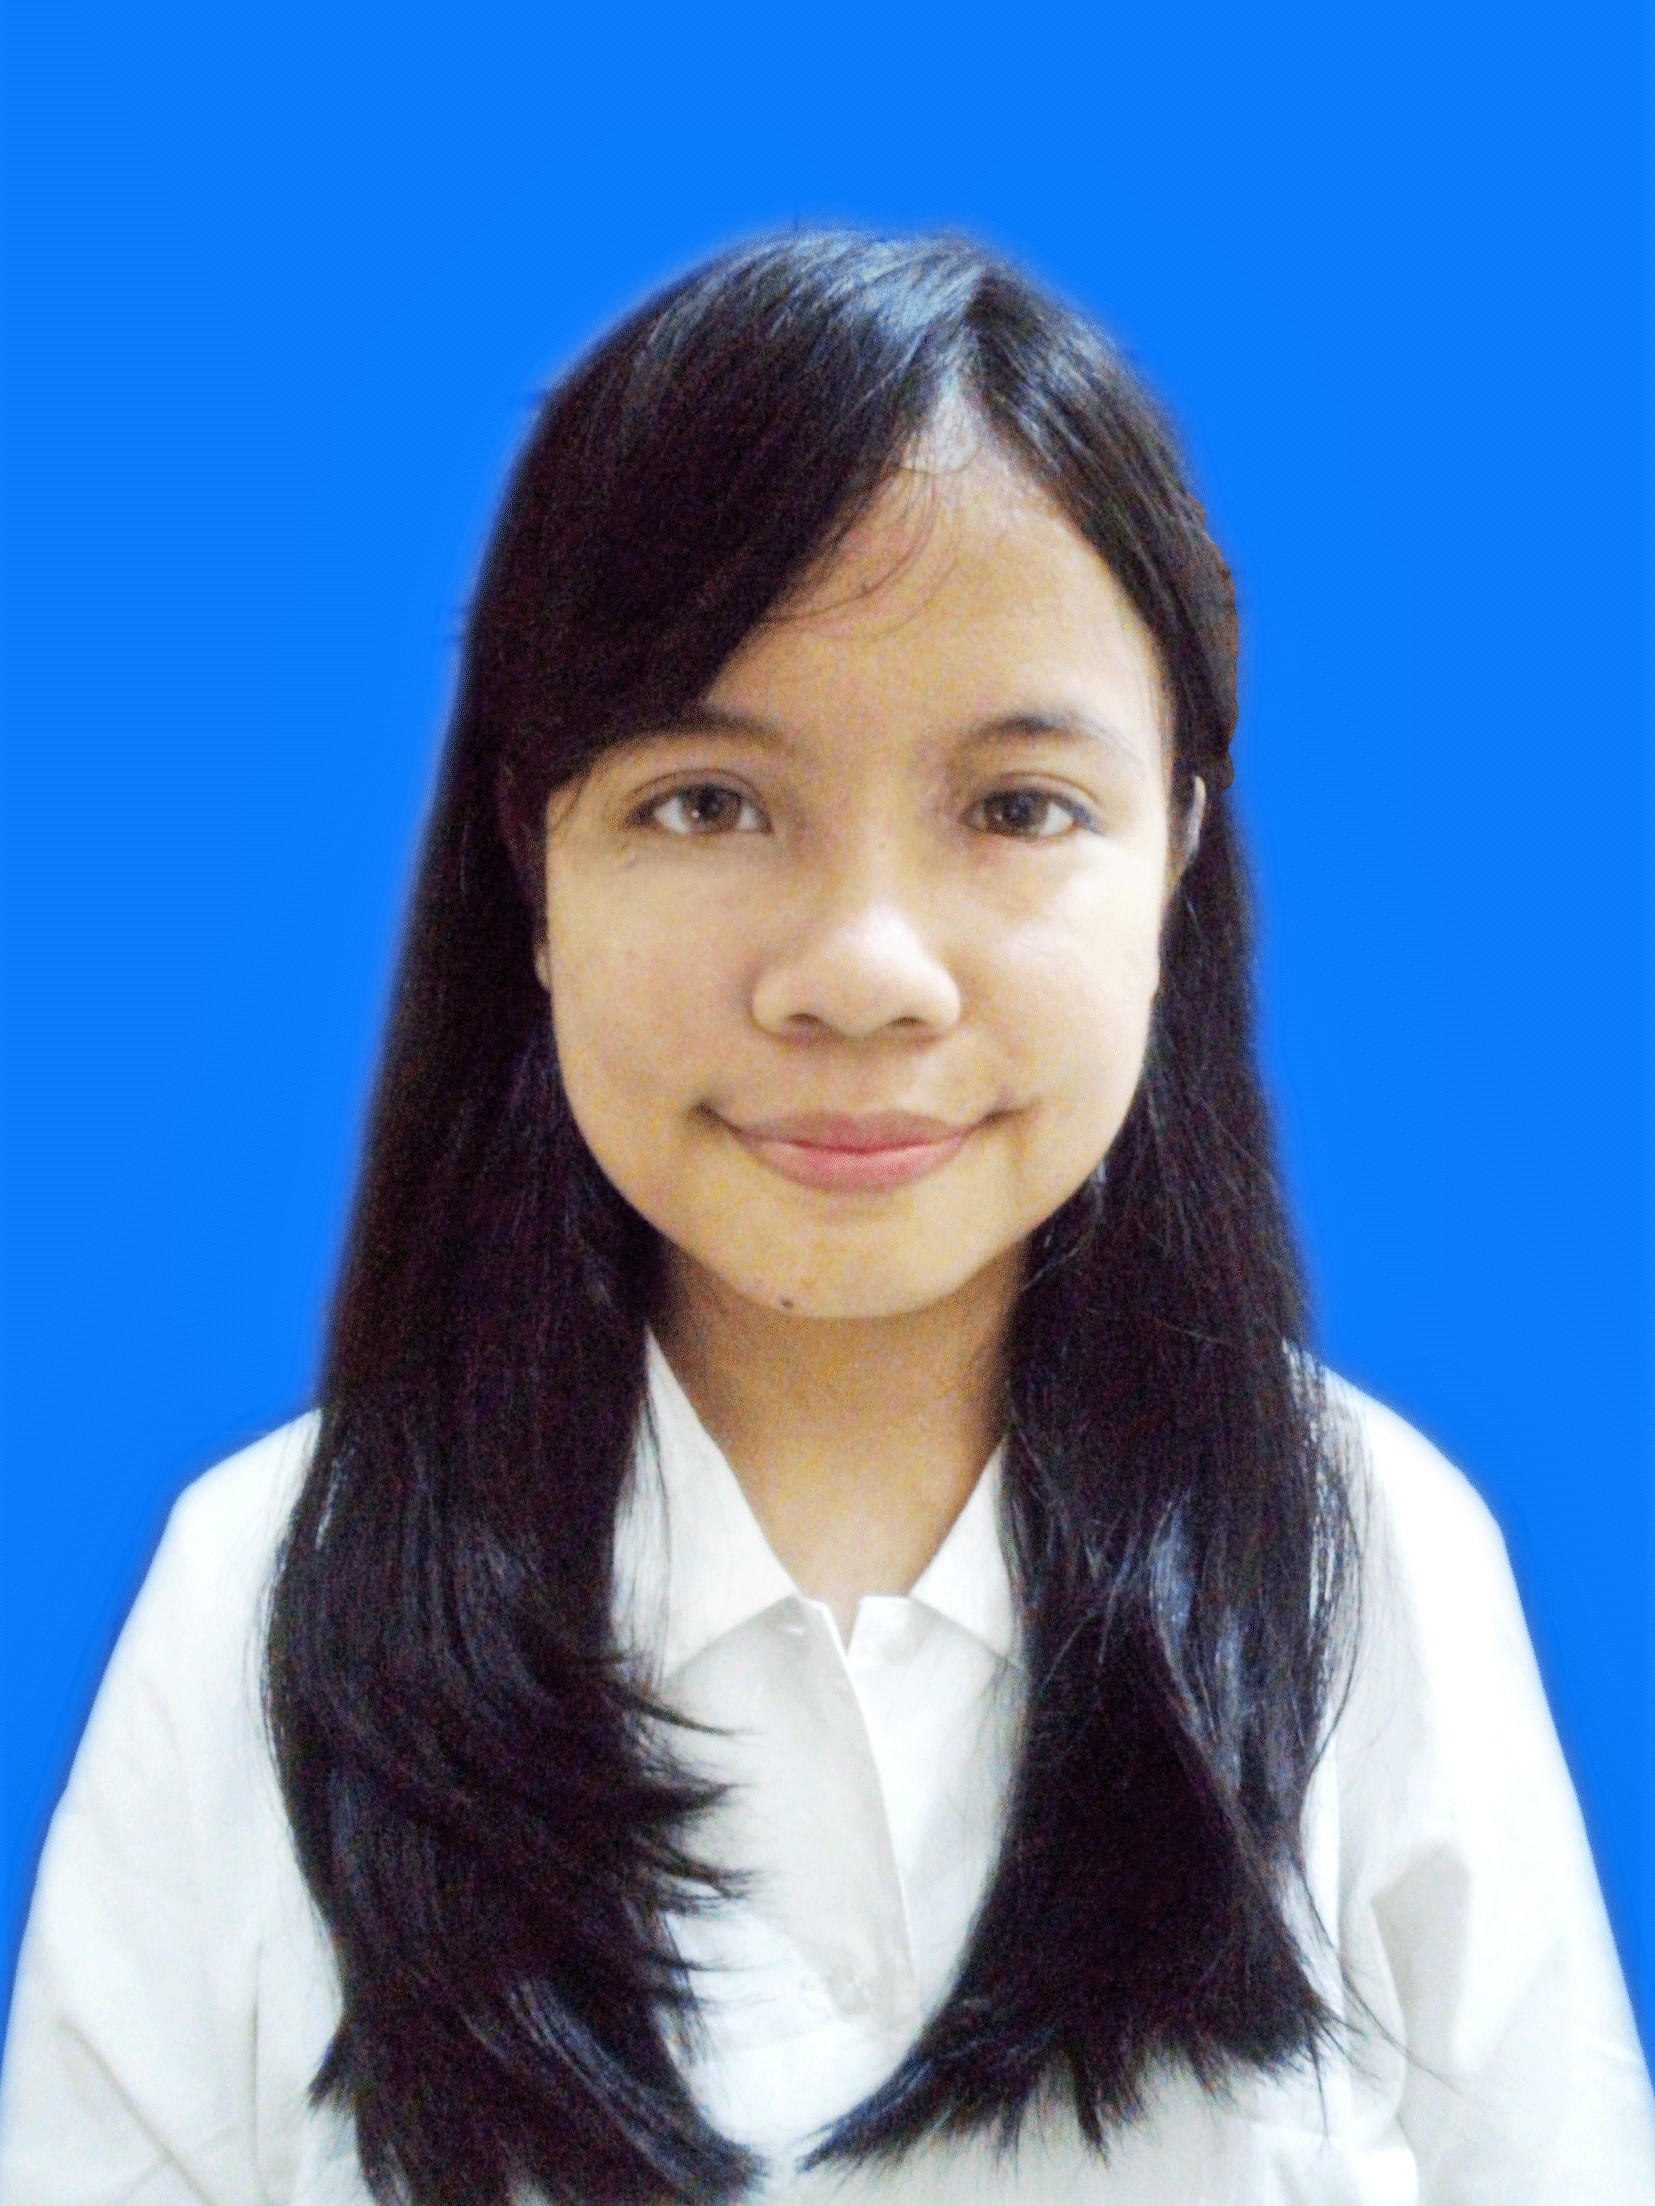
\includegraphics[width=1in,height=1.25in,clip,keepaspectratio]{picture}}]{Ronauli Silva}
\blindtext
\end{IEEEbiography}
% let's finish this
% happily
\end{document}


